% !TeX encoding = UTF-8

\documentclass{protokol}


\usepackage{tikz}
\usetikzlibrary{calc}
\usetikzlibrary{arrows}

%====== Units =====
\usepackage{siunitx}
\sisetup{inter-unit-product =\ensuremath{\cdot}}
\sisetup{group-digits = integer}
\sisetup{output-decimal-marker = {,}}
\sisetup{exponent-product = \ensuremath{\cdot}}
\sisetup{separate-uncertainty}
\sisetup{tight-spacing = false}
%\sisetup{scientific-notation = true}
%\sisetup{round-mode=places,round-precision=4}
%\sisetup{evaluate-expression}


%====== Grafy =====
\usepackage{pgfplots}
\pgfplotsset{width=0.8\linewidth, compat=1.17}
\def\plotcscale{0.8}
\usepackage{pgfplotstable}
\usepackage[figurename=Obr.]{caption} % figure caption rename

%====== Rovnice align block ======
\usepackage{amsmath}
\setlength{\jot}{10pt} % rozestup mezi řádky

\graphicspath{ {./img/} }

%====== Vyplňte údaje ======
\jmeno{Jakub Charvot}
\kod{240844}
\rocnik{2.}
\obor{MET}
\skupina{MET/2}
\spolupracoval{--}

\merenodne{--}
\odevzdanodne{4.5.\ 2023}
\nazev{Laditelná dolní propust s~AD633}
\cislo{38} %měřené úlohy

\predmet{Modelování a~počítačová simulace}
\ustav{Ústav mikroelektroniky}
\skola{FEKT VUT v~Brně}

\def\para{x+0}
\def\parb{\para-80}


%citace 
\usepackage[backend=biber, style=iso-numeric, sortlocale=cs_CZ, autolang=other, language=czech]{biblatex}
\addbibresource{bibliography.bib}
\DeclareFieldFormat{labelnumberwidth}{\mkbibbrackets{#1}}
% hyperlinky
\usepackage[colorlinks]{hyperref}

% odstavce
\usepackage{parskip}

% Bloky kódu
\usepackage{xcolor}

%New colors defined below
\definecolor{codegreen}{rgb}{0,0.6,0}
\definecolor{codegray}{rgb}{0.5,0.5,0.5}
\definecolor{codepurple}{rgb}{0.58,0,0.82}
\definecolor{backcolour}{rgb}{0.95,0.95,0.92}

\usepackage{listings}
\lstdefinestyle{mystyle}{
  backgroundcolor=\color{backcolour}, commentstyle=\color{codegreen},
  keywordstyle=\color{magenta},
  numberstyle=\tiny\color{codegray},
  stringstyle=\color{codepurple},
  basicstyle=\ttfamily\footnotesize,
  breakatwhitespace=false,         
  breaklines=true,                 
  captionpos=b,                    
  keepspaces=true,                 
  numbers=left,                    
  numbersep=5pt,                  
  showspaces=false,                
  showstringspaces=false,
  showtabs=false,                  
  tabsize=2
}
\lstset{
	inputencoding=utf8,
	extendedchars=true,
	literate={á}{{\'a}}1 {č}{{\v{c}}}1 {ď}{{\v{d}}}1 {é}{{\'e}}1 {ě}{{\v{e}}}1 
           {í}{{\'i}}1 {ň}{{\v{n}}}1 {ó}{{\'o}}1 {ř}{{\v{r}}}1 {š}{{\v{s}}}1 
           {ť}{{\v{t}}}1 {ú}{{\'u}}1 {ů}{{\r{u}}}1 {ý}{{\'y}}1 {ž}{{\v{z}}}1 
           {Á}{{\'A}}1 {Č}{{\v{C}}}1 {Ď}{{\v{D}}}1 {É}{{\'E}}1 {Ě}{{\v{E}}}1 
           {Í}{{\'I}}1 {Ň}{{\v{N}}}1 {Ó}{{\'O}}1 {Ř}{{\v{R}}}1 {Š}{{\v{S}}}1 
           {Ť}{{\v{T}}}1 {Ú}{{\'U}}1 {Ů}{{\r{U}}}1 {Ý}{{\'Y}}1 {Ž}{{\v{Z}}}1,
	style=mystyle
	}

% Číslování
\pagenumbering{arabic}



% =========================================
% =============== DOKUMENT ================
% =========================================
\begin{document}
	%====== Vygenerování tabulky ======
	\maketitle

\section*{Úvod}
	Tento projekt se zabývá analýzou analogové násobičky AD633 ve funkci laditelné dolní propusti v~prostředí SPICE. Studentká verze programu PSpice~\cite{cadence} má bohužel omezenou funkcionalitu a~také v~prostředí Linux, které autor tohoto projektu používá, nefunguje bezchybně, proto byl pro vypracování použit zejména program Ngspice~\cite{ngspice}, což je jedna z~open-source variant programu SPICE. Ngspice má také různé rozšiřující možnosti zápisu, které podle názoru autora této práce dělají kód o něco přehlednější, ale bohužel není zpětně kompatibilní s~PSpice.

	Celý zdrojový kód použitý pro simulace v~tomto projektu se nachází v~příloze~\ref{priloha:projekt.cir}. Ngspice kromě výstupních souborů umožňuje také generovat data přímo do souborů typu CSV, což umožňuje následné snadné další zpracování dat, zde vykreslení do grafu v~prostředí LaTeX.
\section{Popis součástky}
	AD633 je analogová čtyřkvadrantová násobička, která se vyznačuje vysokou přesností a~linearitou na celém pracovním rozsahu. Při vhodném zapojení umožňuje použití v~různých aplikacích: přesné analogové násobení a~dělení signálů, odmocnina, násobička kmitočtu, řízená horní nebo dolní propust (která je tématem této práce) a~mnohé další~\cite{ad633datasheet}.

	\begin{figure}[h!]
		\centering
		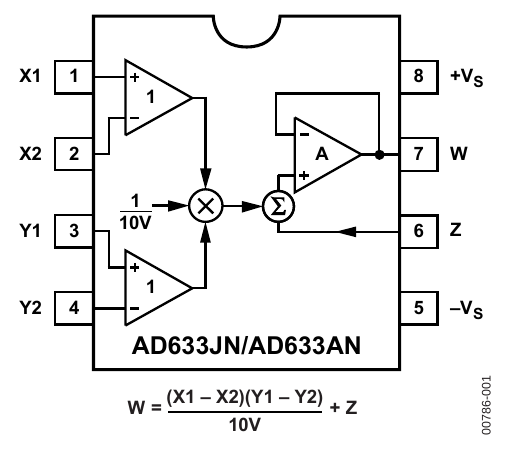
\includegraphics[width=0.5\textwidth]{img/ad633.png}
		\caption{Rozložení vývodů a~blokové schéma násobičky AD633. Převzato z~\cite{ad633datasheet}.}
		\label{fig:img-ad633.png}
	\end{figure}
	
	Součástka má 8 pinů a~může pracovat v~rozmezí napájecího napětí \(\pm 8\)  až  \(\pm 18\) V~\cite{ad633datasheet}. Má dvě dvojice plně diferenciálních vysokoimpedančních vstupů (X1, X2 a~Y1, Y2), k~tomu přičítací vstup Z. Výstup W je pak úměrný součinu napětí na vstupech s~přičtenou hodnotou vstupu Z, ta je vždy přidružena k~výsledku násobení (vizte vztah pro W na Obr.~\ref{fig:img-ad633.png}).

\section{SPICE model}
	Model SPICE, použitý v~tomto projektu byl získán přímo z~webu společnosti Analog devices~\cite{spicemodel}, která je výrobcem této součástky. Jedná se o poslední revizi z~15.9. 2014. 

	Pořadí vývodu je v~modelu nastaveno stejně jako na Obr.~\ref{fig:img-ad633.png}. Celý kód použitého modelu je k~dispozici v~příloze~\ref{priloha:spicemodel}, se samotným modelem nebyly prováděny žádné změny.

\section{Testované zapojení}
	\begin{figure}[h!]
		\centering
		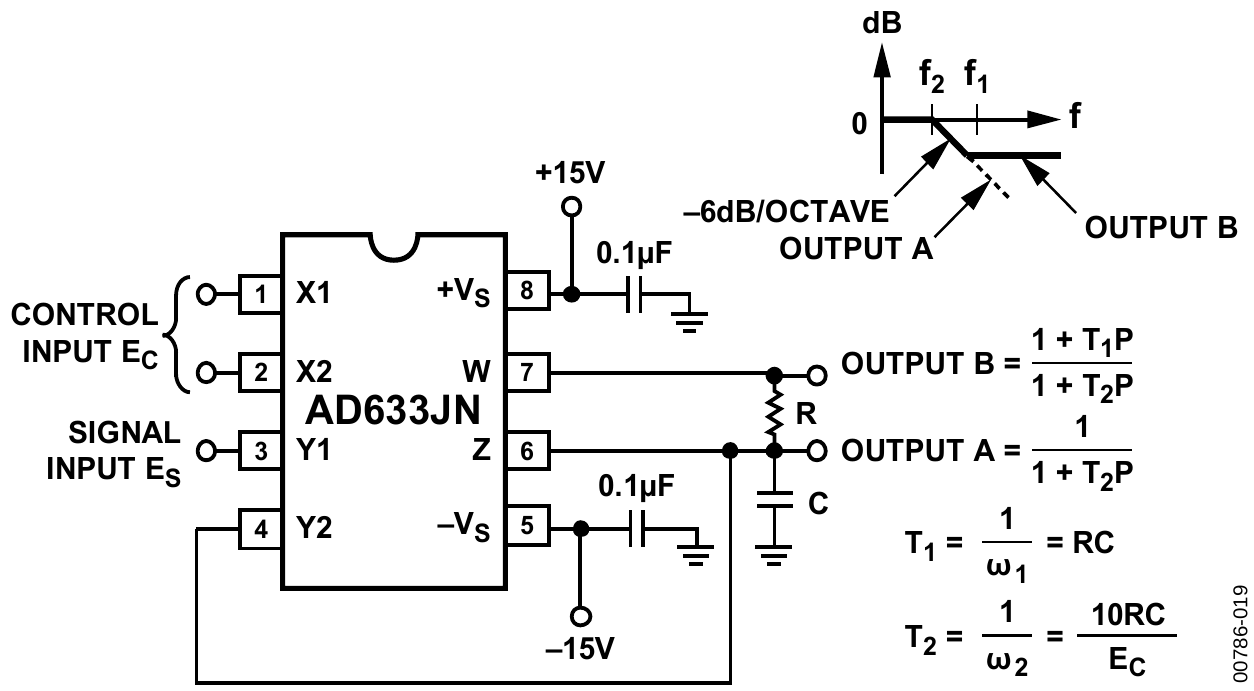
\includegraphics[width=0.8\textwidth]{img/schema.png}
		\caption{Schéma doporučeného zapojení napětím řízeného filtru typu DP. Převzato z~\cite{ad633datasheet}.}
		\label{fig:img-schema-png}
	\end{figure}

	V tomto zapojení (Obr.~\ref{fig:img-schema-png}) je na vstup Y1 (značeno \(E_{S} \) ) přiveden vstupní signál, který chceme filtrovat. Výsledek filtrace je pak na svorce z~(značeno OUTPUT A), což není přímo výstup obvodu AD633 a~je tedy zatížen vyšší výstupní impedancí, v~závislosti na aplikaci může být potřeba připojit zde ještě sledovač.


	Alternativně lze využít také výstup W (značeno OUTPUT B), který má nízkou výstupní impedanci a~lze jej tedy více zatížit. Na nižších frekvencích se chová stejně, od frekvence \(f_{2} \) už ale přestává růst jeho zeslabovací funkce a~zeslabení zůstává na konstantní úrovni, znázornění ideální přenosové funkce tohoto filtru je opět na Obr.~\ref{fig:img-schema-png}.

	Horní mezní frekvenci \(f_{2} \) filtru a~také již zmíněnou frekvenci \(f_{1} \) lze určit následovně:
	\[
		f_{2} =\frac{E_{C} }{10(2\pi RC)}
	\]
	\[
		f_{1} =\frac{1}{2\pi RC}
	\]
	Z uvedených vztahů je vidět, že vlastnosti filtru jsou závislé na hodnotách součástek R a~C a~také na řídícím napětí \(E_{C} \).
	
	Vhodnou volbou hodnot součástek lze dosáhnout možnosti regulace mezní frekvence v~námi požadovaném rozsahu pouze za pomocí napětí \(E_{C} \). 

\clearpage
\section{Prováděné simulace}
	Jak již bylo zmíněno v~úvodu, v~této  práci byl využíván zejména program Ngspice, ten oproti klasické syntaxi PSpice umožňuje využít sekci \textit{.control}, ve které je možné provádět různé typy simulací, za běhu měnit hodnoty součástek nebo parametrů a~také využívat příkazy podmínek a~cyklů. Díky tomu je možné všechny simulace v~tomto projektu spustit v~rámci jednoho běhu programu. 
	
	Celý použitý zdrojový kód se nachází v~příloze~\ref{priloha:projekt.cir}, případně je k dispozici také veřejně ve formě github repozitáře~\cite{github-repo}, společně se zdrojovým kódem pro LaTeX a vygenerovanými CSV soubory.

	\subsection{Závislost amplitudových kmitočtových charakteristik na řídícím napětí \(E_{C}\)}
		Jak je již zmíněno v~předchozí sekci, kmitočtová charakteristika filtru s~AD633 je závislá na třech proměnných: Hodnotách součástek R a~C a~velikosti řídícího napětí \(E_{C} \). 
		
		Pro účely této simulace byly zvoleny hodnoty R=\qty{10}{\kilo\ohm} a~C=\qty{1}{\nano\farad}, které se dále neměnily a~bylo pracováno pouze s~velikostí řídícího napětí. Tyto hodnoty byly zvoleny po několika pokusech, poněvadž umožňují dosáhnout nejlepších výsledků při nastavování mezní frekvence filtru v~akustickém pásmu frekvencí, což bylo cílem stanoveným autorem této práce.
		
		V zadání projektu je specifikováno, že mají být simulována pouze kladná napětí, byly tedy voleny hodnoty v~rozsahu od 0 do \qty{15}{\volt}, což je velikost připojeného napájecího napětí a~tedy dle katalogového listu~\cite{ad633datasheet} i~maximální hodnota \(E_{C} \). Výsledky simulace jsou zobrazeny na Obr.~\ref{graf-simulace-Ec}.

		\begin{figure*}[h!]
			\begin{tikzpicture}
				\centering
				\begin{axis}
					[
					xlabel={\( f\ [\unit{Hz}]\)},
					ylabel={\( K\ [\unit{dB}]\)},
					%axis y line*=left, % dve y osy
					width=1\textwidth,
					height = 0.5\textwidth,
					legend pos=south west,
					legend style={draw=none},
					legend cell align={left},
					xmin=1,
					% ymin=-5,
					xmax=1e6,
		%			ymax=100
					xmode=log
					]
					\addplot[mark=none, mark options={solid}, thick, blue, solid, mark size=3pt] table [skip first n=0, x=frequency, y=db(v(Z)), col sep=space] {data/d/outputec-0+.csv};
					\addlegendentry{\(E_{C}\)=\qty{0}{\volt}}
					\addplot[mark=none, mark options={solid}, thick, cyan, solid, mark size=3pt] table [skip first n=0, x=frequency, y=db(v(Z)), col sep=space] {data/d/outputec-10m+.csv};
					\addlegendentry{\(E_{C}\)=\qty{10}{\milli\volt}}
					\addplot[mark=none, mark options={solid}, thick, red, solid, mark size=3pt] table [skip first n=0, x=frequency, y=db(v(Z)), col sep=space] {data/d/outputec-100m+.csv};
					\addlegendentry{\(E_{C}\)=\qty{100}{\milli\volt}}
					\addplot[mark=none, mark options={solid}, thick, green, solid, mark size=3pt] table [skip first n=0, x=frequency, y=db(v(Z)), col sep=space] {data/d/outputec-1+.csv};
					\addlegendentry{\(E_{C}\)=\qty{1}{\volt}}
					\addplot[mark=none, mark options={solid}, thick, black, solid, mark size=3pt] table [skip first n=0, x=frequency, y=db(v(Z)), col sep=space] {data/d/outputec-10+.csv};
					\addlegendentry{\(E_{C}\)=\qty{10}{\volt}} 
					\addplot[mark=none, mark options={solid}, thick, black, dashed, mark size=3pt] table [skip first n=0, x=frequency, y=db(v(Z)), col sep=space] {data/d/outputec-15+.csv};
					\addlegendentry{\(E_{C}\)=\qty{15}{\volt}} 			
			\end{axis} 
			\end{tikzpicture}
			\caption{Síť amplitudových kmitočtových charakteristik v~závislosti na řídícím napětí \(E_{c} \). Simulováno v Ngspice~\cite{ngspice}.}
			\label{graf-simulace-Ec}
		\end{figure*}


		Z grafu je patrné, že pro velmi malé řídící napětí je mezní frekvence filtru téměř nulová a~i pro stejnosměrnou složku dochází k~poklesu o několik dB, naopak pro řídící napětí od zhruba \qty{80}{\milli\volt} můžeme nastavovat mezní frekvenci v~akustickém pásmu.
	
	\clearpage
	\subsection{Teplotní závislost}
		Dále byl zkoumán vliv teploty na tento obvod. Pro všechny simulace platí, že jsou vztaženy k~normované teplotě \(T_{NORM} \) =\qty{27}{\degreeCelsius}. Nejprve byly zkoumány vlastnoti samotného obvodu s~teplotně nezávislými okolními součástkami, výsledky tohoto pokusu lze vidět na Obr.~\ref{graf:teplota-jen-obvod}.
		
		\begin{figure*}[h!]
			\begin{tikzpicture}
				\centering
				\begin{axis}
					[
					xlabel={\( f\ [\unit{Hz}]\)},
					ylabel={\( K\ [\unit{dB}]\)},
					%axis y line*=left, % dve y osy
					yticklabel style={
						/pgf/number format/fixed,
						/pgf/number format/1000 sep=\thinspace % optional if you want to replace comma as the 1000 separator with a thin space
					  },
					scaled ticks=false,
					width=1\textwidth,
					height = 0.5\textwidth,
					legend pos=south west,
					legend style={draw=none},
					legend cell align={left},
					xmin=10,
					% ymin=1,
					xmax=1e3,
					%			ymax=100
					xmode=log
					]
					\addplot[mark=none, mark options={solid}, thick, cyan, solid, mark size=3pt] table [skip first n=0, x=frequency, y=db(v(Z)), col sep=space] {data/d-teplota1/outputtemp-0+.csv};
					\addlegendentry{T=\qty{0}{\degreeCelsius}}
					\addplot[mark=none, mark options={solid}, thick, blue, solid, mark size=3pt] table [skip first n=0, x=frequency, y=db(v(Z)), col sep=space] {data/d-teplota1/outputtemp-20+.csv};
					\addlegendentry{T=\qty{20}{\degreeCelsius}}
					\addplot[mark=none, mark options={solid}, thick, red, solid, mark size=3pt] table [skip first n=0, x=frequency, y=db(v(Z)), col sep=space] {data/d-teplota1/outputtemp-40+.csv};
					\addlegendentry{T=\qty{40}{\degreeCelsius}}
					\addplot[mark=none, mark options={solid}, thick, green, solid, mark size=3pt] table [skip first n=0, x=frequency, y=db(v(Z)), col sep=space] {data/d-teplota1/outputtemp-60+.csv};
					\addlegendentry{T=\qty{60}{\degreeCelsius}}
					\addplot[mark=none, mark options={solid}, thick, orange, solid, mark size=3pt] table [skip first n=0, x=frequency, y=db(v(Z)), col sep=space] {data/d-teplota1/outputtemp-80+.csv};
					\addlegendentry{T=\qty{80}{\degreeCelsius}}
					\addplot[mark=none, mark options={solid}, thick, black, solid, mark size=3pt] table [skip first n=0, x=frequency, y=db(v(Z)), col sep=space] {data/d-teplota1/outputtemp-100+.csv};
					\addlegendentry{T=\qty{100}{\degreeCelsius}}
					
				\end{axis} 
			\end{tikzpicture}
			\caption{Teplotní závislost amplitudové kmitočtové charakteristiky pro \(E_{c}  \) = \qty{100}{\milli\volt}. Simulováno v Ngspice~\cite{ngspice}.}
			\label{graf:teplota-jen-obvod}
		\end{figure*}

		V obvodu opravdu nastaly v~závislosti na teplotě drobné změny, ale jsou natolik malé, že je v~grafu nelze ani okem rozlišit. V~popisu SPICE modelu, který byl v~této práci použit, bohužel není uvedeno, jestli je určený i~pro teplotní analýzu. Ani v~katalogovém listu jsem informaci o tepelné závislosti nenašel, lze tedy předpokládat, že samotný obvod bude zřejmě proti změnám teploty vcelku odolný. 

		
		\begin{figure*}[h!]
			\begin{tikzpicture}
				\centering
				\begin{axis}
					[
						xlabel={\( f\ [\unit{Hz}]\)},
						ylabel={\( K\ [\unit{dB}]\)},
						%axis y line*=left, % dve y osy
						width=1\textwidth,
						height = 0.5\textwidth,
						legend pos=south west,
						legend style={draw=none},
						legend cell align={left},
						xmin=10,
						% ymin=1,
						xmax=1e3,
						%			ymax=100
						xmode=log
						]
						\addplot[mark=none, mark options={solid}, thick, cyan, solid, mark size=3pt] table [skip first n=0, x=frequency, y=db(v(Z)), col sep=space] {data/d-teplota2/outputtemp-0+.csv};
						\addlegendentry{T=\qty{0}{\degreeCelsius}}
						\addplot[mark=none, mark options={solid}, thick, blue, solid, mark size=3pt] table [skip first n=0, x=frequency, y=db(v(Z)), col sep=space] {data/d-teplota2/outputtemp-20+.csv};
						\addlegendentry{T=\qty{20}{\degreeCelsius}}
						\addplot[mark=none, mark options={solid}, thick, red, solid, mark size=3pt] table [skip first n=0, x=frequency, y=db(v(Z)), col sep=space] {data/d-teplota2/outputtemp-40+.csv};
						\addlegendentry{T=\qty{40}{\degreeCelsius}}
						\addplot[mark=none, mark options={solid}, thick, green, solid, mark size=3pt] table [skip first n=0, x=frequency, y=db(v(Z)), col sep=space] {data/d-teplota2/outputtemp-60+.csv};
						\addlegendentry{T=\qty{60}{\degreeCelsius}}
						\addplot[mark=none, mark options={solid}, thick, orange, solid, mark size=3pt] table [skip first n=0, x=frequency, y=db(v(Z)), col sep=space] {data/d-teplota2/outputtemp-80+.csv};
						\addlegendentry{T=\qty{80}{\degreeCelsius}}
						\addplot[mark=none, mark options={solid}, thick, black, solid, mark size=3pt] table [skip first n=0, x=frequency, y=db(v(Z)), col sep=space] {data/d-teplota2/outputtemp-100+.csv};
						\addlegendentry{T=\qty{100}{\degreeCelsius}}
						
					\end{axis} 
				\end{tikzpicture}
				\caption{Teplotní závislost amplitudové kmitočtové charakteristiky pro \(E_{c}  \) = \qty{100}{\milli\volt}, TC1=\qty{3000}{ppm} pro R a~C. Simulováno v Ngspice~\cite{ngspice}.}
				\label{graf:teplota-soucastky}
			\end{figure*}
			
			Ve druhém scénáři byla součástkám R a~C přidána teplotní závislost (lineární teplotní součinitel odporu/kapacity \qty{3000}{ppm}), výsledky jsou zobrazeny na Obr.~\ref{graf:teplota-soucastky}. Zde je už závislost výraznější, s~rostoucí teplotou mírně klesá mezní frekvence filtru, tedy při návrhu obvodu s~tímto zapojením by měl vývojář mít tuto informaci na paměti a~volit součástky s~dostatečně nízkým teplotním koeficientem.

	% \clearpage
	\subsection{Závislost horního mezního kmitočtu filtru na velikosti \(E_{C} \) }
		Z rovnice uvedené výše lze stanovit hodnotu horní mezní frekvence filtru (\(f_{2} \)), pro zvolené konstantní hodnoty součástek (R=\qty{10}{\kilo\ohm}, C=\qty{1}{\nano\farad}) nám vznikne lineární závislost:
		\[
			f_{2} =\frac{E_{C} }{10(2\pi RC)} = E_{C} \cdot \frac{1}{20\pi\cdot \num{10e3}\cdot \num{1e-9}}\approx 1591\cdot E_{C} 
		\]
		\begin{figure*}[h!]
			\begin{tikzpicture}
				\centering
				\begin{axis}
					[
					xlabel={\( E_{c} \ [\unit{V}]\)},
					ylabel={\( f_{2} \ [\unit{kHz}]\)},
					yticklabel style={
						/pgf/number format/fixed,
						/pgf/number format/1000 sep=\thinspace % optional if you want to replace comma as the 1000 separator with a thin space
					  },
					scaled ticks=false,
					y filter/.code={\pgfmathparse{#1/1000}\pgfmathresult},
					width=1\textwidth,
					height = 0.5\textwidth,
					legend pos=south east,
					legend style={draw=none},
					legend cell align={left},
		%			xmin=0,
		%			ymin=0,
		%			xmax=100
		%			ymax=100
					% ymode=log
					]
					\addplot[mark=none, mark options={solid}, thick, blue, solid, mark size=3pt] table [skip first n=0, x=const.Ec_actual, y=const.f_mez, col sep=space] {data/e/output.csv};
					\addlegendentry{Teoretická křivka}
					\addplot[mark=x, mark options={solid}, thick, red, only marks, mark size=3pt] table [skip first n=0, x=Ec_actual, y=f_mez, col sep=space] {data/e/rucne-z-d.csv};
					\addlegendentry{Ručně odečtené body z~předchozí simulace}
					\addplot[mark=+, mark options={solid}, thick, green, only marks, mark size=3pt] table [skip first n=0, x=const.Ec_actual, y=const.lastFreq, col sep=space] {data/e/output.csv};
					\addlegendentry{Automatická detekce z~AC simulace}
			\end{axis} 
			\end{tikzpicture}
			\caption{Závislost mezní frekvence na řídícím napětí. Simulováno v Ngspice~\cite{ngspice}.}
			\label{graf:mezni-frekvence-na-napeti}
		\end{figure*}

		Na Obr.~\ref{graf:mezni-frekvence-na-napeti} můžeme vidět, že ručně odečtené hodnoty mezní frekvence (v datech z~prvního měření byly pro jednotlivá řídící napětí vyhledány frekvence, kterým odpovídá přenos \qty{-3}{dB}) odpovídají uvedené rovnici, lze se tedy podle ní řídit. K~odchylkám dochází až při hodnotách blížících se maximálnímu povolenému napětí.
		
		Pro lepší citlivost a~opakovatelnost měření byla nakonec vytvořena vlastní funkce pro automatickou detekci mezní frekvence z~dat AC simulace \footnote{V ngspice se tato funkce standartně nenachází nebo nebyla autorem této práce nalezena.} a~byla provedena simulace pro vyšší množství hodnot \(E_{C} \). Výsledky podpořily předchozí odhad a~jsou opět viditelné na Obr.~\ref{graf:mezni-frekvence-na-napeti}.

	\clearpage
	\subsection{Vlastní experiment: zkreslení signálu}
	\label{sekce:vlastni-experiment}
		Cílem tohoto experimentu bylo zjistit, jestli po průchodu signálu filtrem dochází k~jeho deformaci popř. fázovému posunu. Namísto analýzy AC tedy bylo provedena analýza TRANSIENT pro různé hodnoty frekvence vstupního harmonického signálu a~následně fourierova analýza pro prvních 10 harmonických složek, z~nich pak program~\cite{ngspice} vypočítal THD \footnote{Činitel harmonického zkreslení, z~anglického total harmonic distortion.}.

		Simulace byla provedena pro hodnoty R=\qty{10}{\kilo\ohm}, C=\qty{1}{\nano\farad}, \(E_{C} \) = \qty{1}{\volt} a~testovány byly frekvence v~propustném i~nepropustném pásmu. Nejvyšší dosažené hodnoty THD byly v~řádu tisícin procenta, tedy obvod AD633 buďto signál téměř nezkresluje a~nebo toto chování není podporováno použitým SPICE modelem~\cite{spicemodel}. Ačkoliv nebylo pozorováno zkreslení výstupního signálu, byl zde patrný fázový posun.
		
		Ke stanovení závislosti fázového posunu byla využita data AC analýzy z~první simulace, ale namísto amplitudových kmitočtových charakteristik byly na Obr.~\ref{graf:simulace-faze} zobrazeny fázové charakteristiky.

		Při porovnání Obr.~\ref{graf-simulace-Ec} a~\ref{graf:simulace-faze} je vidět, že v~propustném pásmu k~fázovému posunu téměř nedochází, po dosažení mezní frekvence už ano, ale tento signál je obecně filtrem potlačen a~tedy fázový posun v~této frekvenční oblasti nečiní velký problém.

		\begin{figure*}[h!]
			\begin{tikzpicture}
				\centering
				\begin{axis}
					[
					xlabel={\( f\ [\unit{Hz}]\)},
					ylabel={\( K\ [\unit{dB}]\)},
					ytick={-3.14,-2.36,-1.57,-0.79,0,0.79,1.57}, % Set y-axis ticks to PI values
    				yticklabels={$-\pi$,$-\frac{3\pi}{4}$,$-\frac{\pi}{2}$,$-\frac{\pi}{4}$,$0$,$\frac{\pi}{4}$,$\frac{\pi}{2}$}, % Set y-axis tick labels to PI values
					%axis y line*=left, % dve y osy
					width=1\textwidth,
					height = 0.5\textwidth,
					legend pos=south west,
					legend style={draw=none},
					legend cell align={left},
					xmin=1,
					% ymin=-5,
					xmax=1e6,
		%			ymax=100
					xmode=log
					]
					\addplot[mark=none, mark options={solid}, thick, blue, solid, mark size=3pt] table [skip first n=0, x=frequency, y=ph(v(Z)), col sep=space] {data/d/outputec-0+.csv};
					\addlegendentry{\(E_{C}\)=\qty{0}{\volt}}
					\addplot[mark=none, mark options={solid}, thick, cyan, solid, mark size=3pt] table [skip first n=0, x=frequency, y=ph(v(Z)), col sep=space] {data/d/outputec-10m+.csv};
					\addlegendentry{\(E_{C}\)=\qty{10}{\milli\volt}}
					\addplot[mark=none, mark options={solid}, thick, red, solid, mark size=3pt] table [skip first n=0, x=frequency, y=ph(v(Z)), col sep=space] {data/d/outputec-100m+.csv};
					\addlegendentry{\(E_{C}\)=\qty{100}{\milli\volt}}
					\addplot[mark=none, mark options={solid}, thick, green, solid, mark size=3pt] table [skip first n=0, x=frequency, y=ph(v(Z)), col sep=space] {data/d/outputec-1+.csv};
					\addlegendentry{\(E_{C}\)=\qty{1}{\volt}}
					\addplot[mark=none, mark options={solid}, thick, black, solid, mark size=3pt] table [skip first n=0, x=frequency, y=ph(v(Z)), col sep=space] {data/d/outputec-10+.csv};
					\addlegendentry{\(E_{C}\)=\qty{10}{\volt}} 
					\addplot[mark=none, mark options={solid}, thick, black, dashed, mark size=3pt] table [skip first n=0, x=frequency, y=ph(v(Z)), col sep=space] {data/d/outputec-15+.csv};
					\addlegendentry{\(E_{C}\)=\qty{15}{\volt}} 			
			\end{axis} 
			\end{tikzpicture}
			\caption{Síť fázových kmitočtových charakteristik v~závislosti na řídícím napětí \(E_{c} \). Simulováno v Ngspice~\cite{ngspice}.}
			\label{graf:simulace-faze}
		\end{figure*}
	
\clearpage
\section*{Reference}
\printbibliography[heading=none]

\clearpage

\section*{Přílohy}

\appendix % příkaz pro začátek sekce příloh
\section{SPICE model \textbf{AD633} (ad633.lib)}
\label{priloha:spicemodel}
\lstinputlisting{../ad633.lib}

\section{Ngspice kód pro simulace v~tomto projektu (projekt.cir)}
\label{priloha:projekt.cir}
\lstinputlisting{../projekt.cir}

\(\) 
\section{Výsledky fourierovy analýzy ve vlastním experimentu (\ref{sekce:vlastni-experiment})}
\label{priloha:fourier-data}
\subsection{\(f_{signal} =\)\qty{10}{\hertz}}
\lstinputlisting{data/f/fourier_output10k+.txt}

\subsection{\(f_{signal} =\)\qty{100}{\hertz}}
\lstinputlisting{data/f/fourier_output100+.txt}

\subsection{\(f_{signal} =\)\qty{1}{\kilo\hertz}}
\lstinputlisting{data/f/fourier_output1k+.txt}

\subsection{\(f_{signal} =\)\qty{10}{\kilo\hertz}}
\lstinputlisting{data/f/fourier_output10+.txt}

\subsection{\(f_{signal} =\)\qty{100}{\kilo\hertz}}
\lstinputlisting{data/f/fourier_output100k+.txt}

\end{document}